\documentclass{article}
\usepackage[utf8]{inputenc}
\usepackage{subcaption}
\usepackage{graphicx}
\usepackage[margin=2.5cm]{geometry}
\usepackage{array}
\usepackage{wrapfig}
\usepackage{multirow}
\usepackage{tabularx}
\usepackage{amsmath}
\usepackage{wrapfig}
\usepackage{mathtools}
\usepackage{gensymb}
\usepackage[table]{xcolor}
\usepackage{xcolor,colortbl}
\usepackage{multirow}
\usepackage{polski}
\title{Sprawozdanie 5\\ Ćwiczenie 48}
\author{Jan Bronicki \\
Nr indeksu: 249011\\
Marcin Radke\\
Nr indeksu: 241554}
\date{}
\begin{document}

\maketitle

\section{Wstęp Teoretyczny}
\par Celem ćwiczenia jest pomiar charakterystyki prądowo-napięciowej różnych diod elektroluminescencyjnych w kierunku przewodzenia oraz wyznaczenie długości fal promieniowania emitowanego przez różnokolorowe diody elektroluminescencyjne.
Na podstawie otrzymanych charakterystyk prądowo-napięciowych możemy wyznaczyć $U_{B}$, dla poszczególnej diody. Dzięki znajomości napięcia $U_{B}$, które jest punktem przecięcia linii prostej wyznaczonej regresji liniowej wziętej z najszybciej rosnącej części wykresu charakterystyki prądowo-napięciowej danej diody oraz $\lambda$ danej diody, czyli długości fali którą emituje. Ze wzoru podanego poniżej możemy obliczyć stałą Plancka $h$:
\vspace{-3ex}
\begin{center}
    $$
    h=\frac{e\cdot \lambda \cdot U_{B}}{c}
    $$
\end{center}
Gdzie:
\par $e$ - ładunek elementarny o wartości $1,6021766208\cdot 10^{−19} C$
\vspace{1.5ex}
\par $c$ - prędkość światła o wartości $ 299 792 458 \frac{m}{s}$\\
\vspace{-2ex}
\begin{flushleft}

Wykaz przyrządów:
\end{flushleft}
\begin{itemize}
    \item Układ zasilający z płynną regulacją napięcia w kierunku przewodzenia i zaporowym
    \item Diody elektroluminescencyjna (czerwona, niebieska i zielona)
    \item Multimetry cyfrowe
    \item Monochromator
    \item Detektor fotooporowy
\end{itemize}


\begin{figure}[h!]
    \centering
    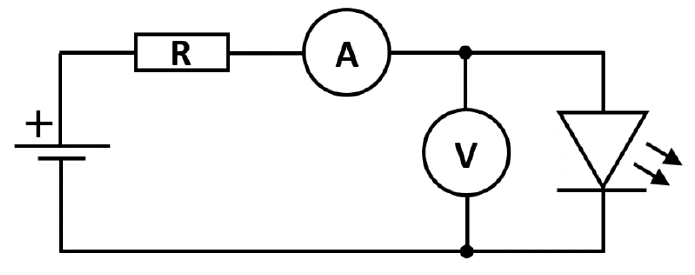
\includegraphics[scale=0.65]{Schemat.PNG}
    \caption{Schemat układu}
\end{figure}

\newpage

\section{Opracowanie Pomiarów}
\begin{figure}[h!]
  \centering
  \begin{subfigure}[b]{0.2\textwidth}
    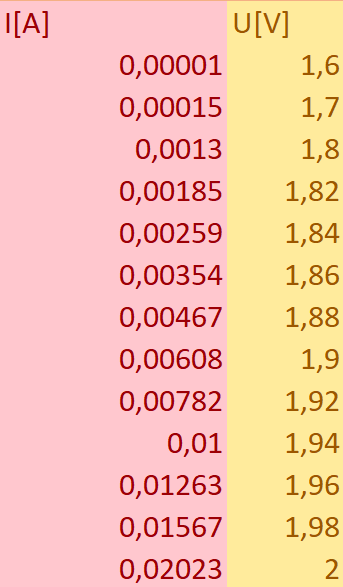
\includegraphics[width=\linewidth]{Pomiary_Dioda_Czerwona.png}
     \caption{Pomiary dioda\\ czerwona}
  \end{subfigure}
  \begin{subfigure}[b]{0.2\textwidth}
    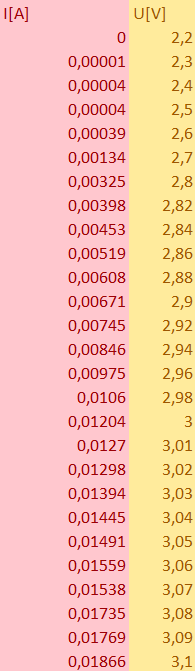
\includegraphics[width=\linewidth]{Pomiary_Dioda_Niebieska.png}
    \caption{Pomiary dioda\\ niebieska}
  \end{subfigure}
  \begin{subfigure}[b]{0.2\textwidth}
    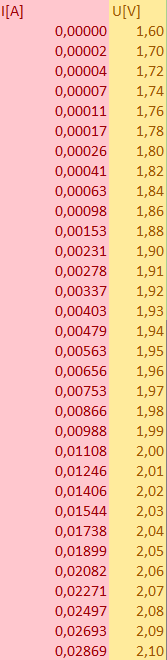
\includegraphics[width=\linewidth]{Pomiary_Dioda_Zielona.png}
    \caption{Pomiary dioda\\ zielona}
  \end{subfigure}
  \caption{Pomiary charakterystyki prądowo-napięciowej, dla diod czerwonej, niebieskiej i zielonej}
\end{figure}
\begin{figure}[h!]
%b
%-0,233806786
%a
%0,126196429
%u(a)
%0,010920933
%u(b)
%0,021191113
    Użyte wzory do obliczania niepewności oraz ich przykładowe obliczenia:\\
    $u_{c}(U_{B})=\sqrt{u^2(b)\cdot \left(\frac{-1}{a}\right)^2+u^2(a)\left(\frac{-b}{a^2}\right)^2}=
    \sqrt{0,022^{2}\cdot \left(\frac{-1}{0,13}\right)^2+0,011^{2}\cdot\left(\frac{0,24}{0,13^2}\right)^2}=0,23 \ V$\\
    
    
    $u(\lambda)=0.01nm=1\cdot 10^{-9}m$\\

    $u_{c}(h)=\sqrt{u^2(\lambda)\cdot\left(\frac{e\cdot U_{B}}{c}\right)^2+u^2(U_{B})\cdot\left(\frac{e\cdot\lambda}{c}\right)^2}
 =
 \sqrt{(1\cdot10^{-11})^2\cdot\left(\frac{1,61\cdot 10^{−19}\cdot 3,51\cdot10^{-35}}{299792458}\right)^2+(0,23)^2\cdot
 \left(\frac{1,61\cdot 10^{−19}\cdot6,12\cdot10^{-7}}{299792458}\right)^2}
 =\\=7,60\cdot10^{-35}
 \left[\frac{m^2kg}{s}\right]$\\
    
    
    $u(I)=\frac{1,4\%\cdot rdg + 3\cdot dgt}{3}=\frac{\frac{1,4}{100}\cdot 0,00001+3\cdot0,00001}{3}=\frac{0,00003014}{3} \approx 0,00001 \ A$\\

    $u(U)=\frac{0,5\%\cdot rdg + 1\cdot dgt}{3}=\frac{\frac{0,5}{100}\cdot 1,6+0,01}{3}=\frac{0,018}{3} \approx 0,01\ V$\\
\end{figure}

\newpage

\begin{flushleft}
Dla diody czerwonej, niebieskiej i zielonej otrzymaliśmy następujące długości fal $\lambda$:
\end{flushleft}
    \par $\lambda_{CZ}=612nm \ \pm0,01nm$
    \vspace{1.5ex}
    \par $\lambda_{N}=440nm \ \pm0,01nm$
    \vspace{1.5ex}
    \par $\lambda_{Z}=585nm \ \pm0,01nm$
    \vspace{1.5ex}


\begin{figure}[b!]
  \centering
  \begin{subfigure}[b]{0.15\textwidth}
    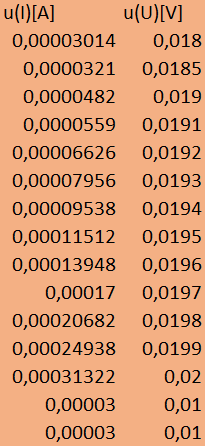
\includegraphics[width=\linewidth]{Niepewnosci_Dioda_Czerwona.png}
     \caption{Niepewności pomiarów, dla diody czerwonej}
  \end{subfigure}
  \begin{subfigure}[b]{0.15\textwidth}
    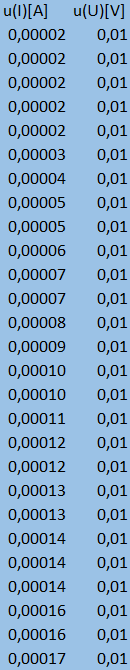
\includegraphics[width=\linewidth]{Niepewnosci_Dioda_Niebieskia.png}
    \caption{Niepewności pomiarów, dla diody niebieskiej}
  \end{subfigure}
  \begin{subfigure}[b]{0.15\textwidth}
    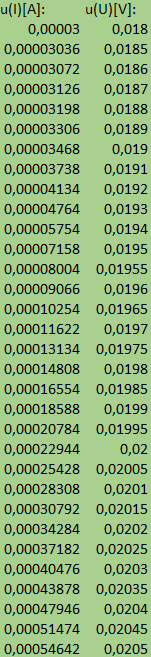
\includegraphics[width=\linewidth]{Niepewnosci_Dioda_Zielona.png}
    \caption{Niepewności pomiarów, dla diody zielonej}
  \end{subfigure}
  \caption{Niepewności pomiarów charakterystyki prądowo-napięciowej, dla diod czerwonej, niebieskiej i zielonej}
\end{figure}
\newpage



\begin{figure}[h]
    \centering
    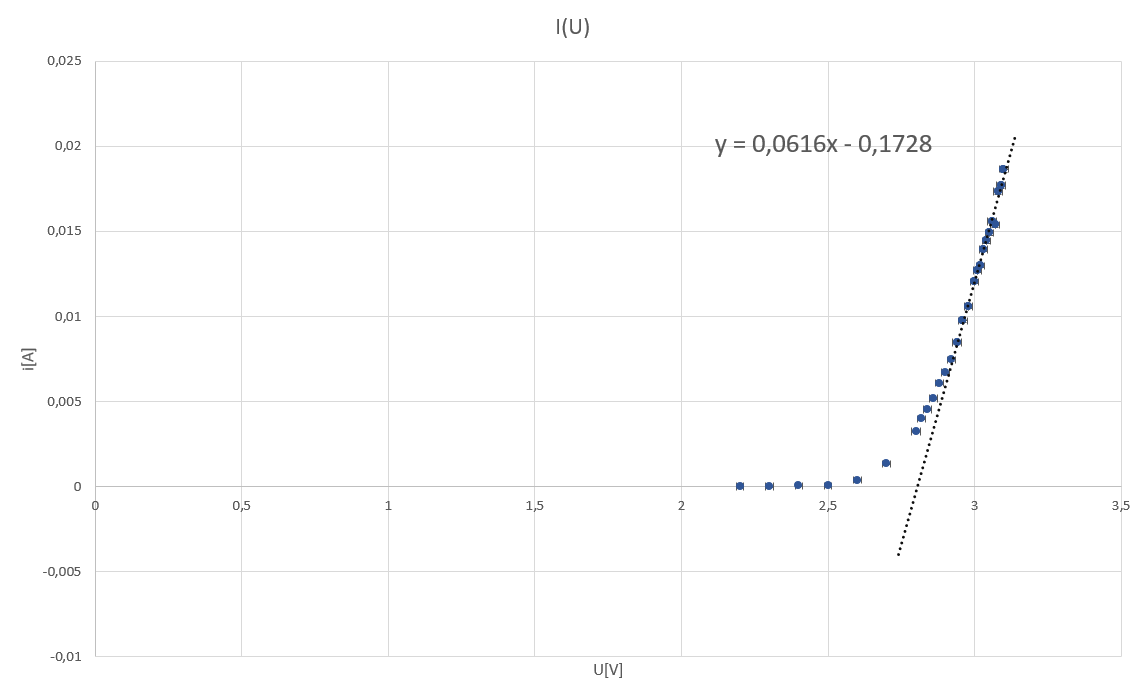
\includegraphics[scale=0.65]{Wykres_Dioda_Niebieska.png}
    \caption{Wykres diody niebieskiej}
\end{figure}
\begin{figure}[h!]
    \centering
    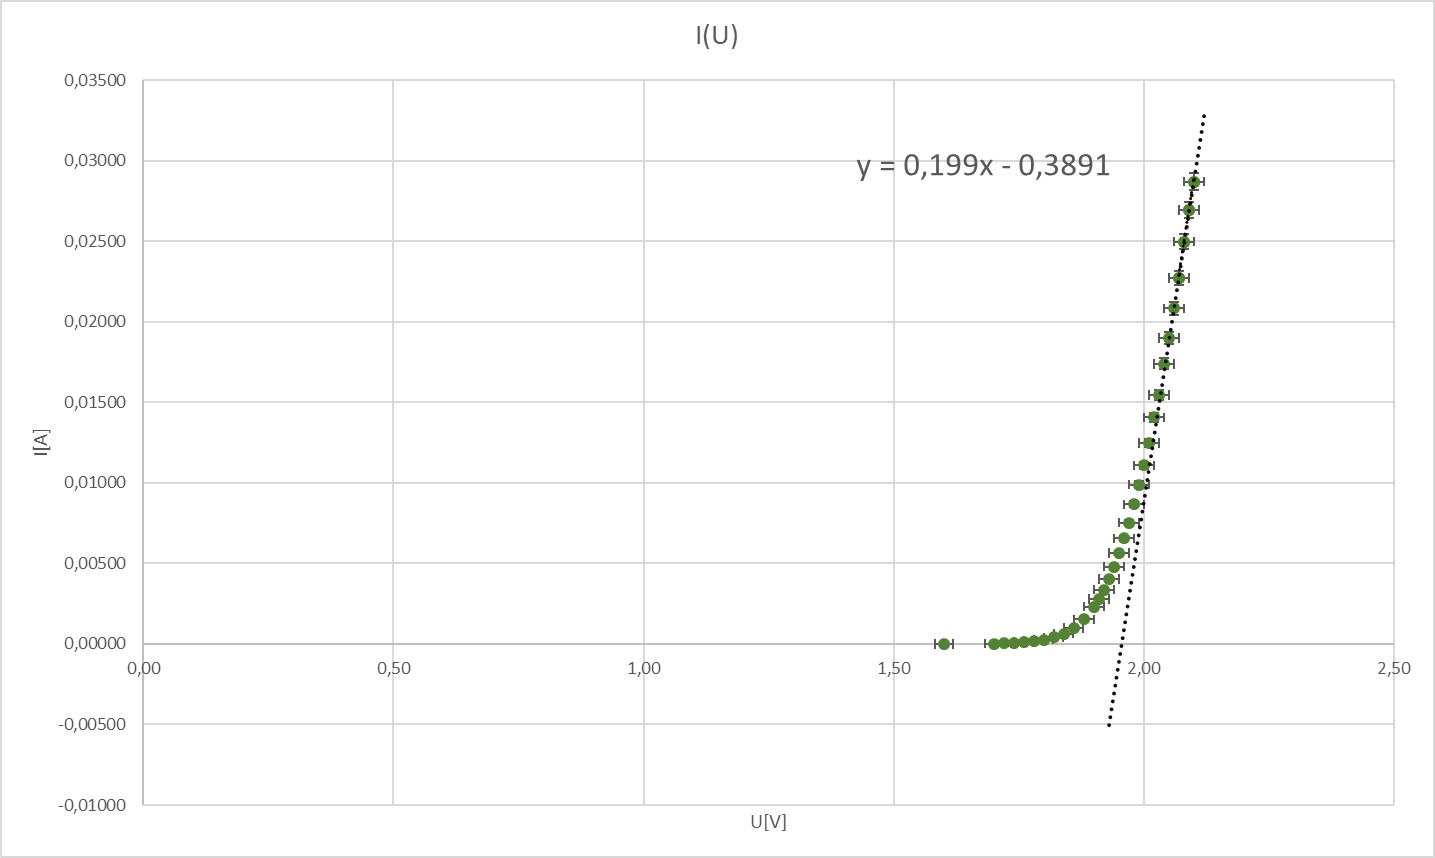
\includegraphics[scale=0.65]{Wykres_Dioda_Zielona.png}
    \caption{Wykres diody zielonej}
\end{figure}
\newpage
\begin{figure}[th!]
    \centering
    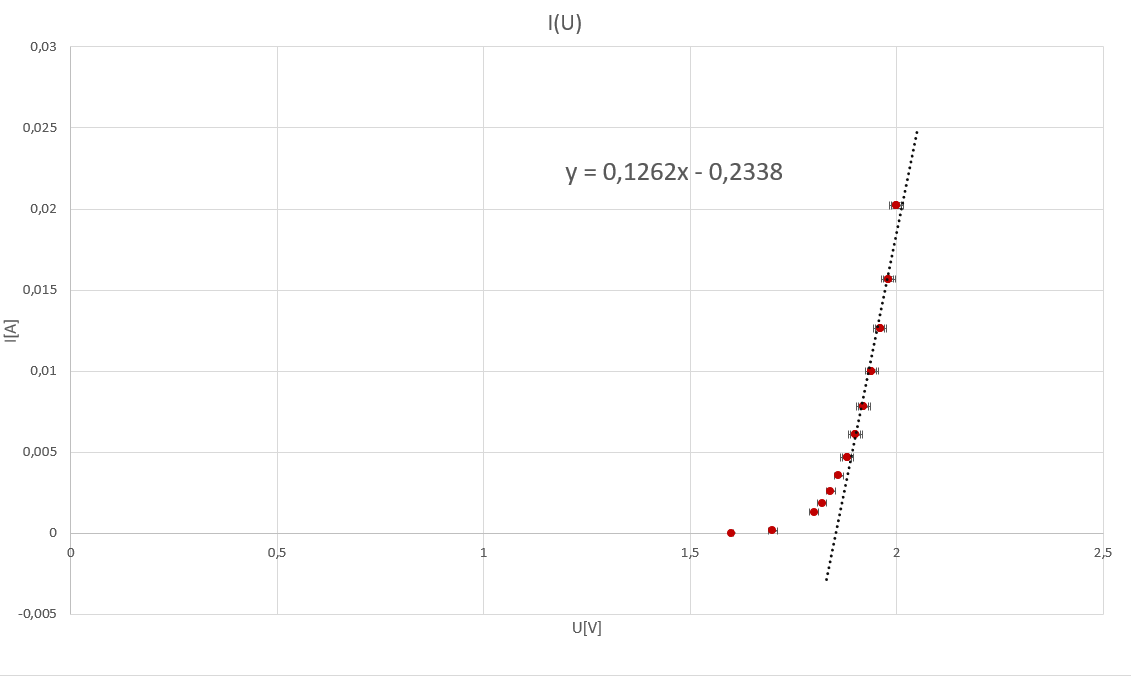
\includegraphics[scale=0.65]{Wykres_Dioda_Czerwona.png}
    \caption{Wykres diody czerwonej}
\end{figure}


\begin{figure}[h!]
    \begin{center}
        Następnie przechodzimy do obliczenia stałych Plankca, dla każdej z diod:
    \end{center}{}
    $$
    h=\frac{e\cdot \lambda \cdot U_{B}}{c}
    $$
    

    \par \ Dioda czerwona:\\ \\
    \vspace{1ex}
    $h_{CZ}=\frac{1,61\cdot 10^{−19}\cdot 6,12\cdot10^{-7} \cdot1,85}{299792458}=6,063\cdot10^{-34} \ \pm0,76\cdot10^{-34} \left[\frac{m^2kg}{s}\right]$\\
    \vspace{2.5ex}
    Dioda niebieska:\\
    \vspace{2ex}
    $h_{N}=\frac{1,61\cdot 10^{−19}\cdot 6,12\cdot10^{-7} \cdot2,81}{299792458}=6,60\cdot10^{-34} \ \pm0,32\cdot10^{-34} \left[\frac{m^2kg}{s}\right]$\\
    \vspace{2ex}
    Dioda zielona:\\
    \vspace{2ex}
    $h_{Z}=\frac{1,61\cdot 10^{−19}\cdot 6,12\cdot10^{-7} \cdot1,96}{299792458}=6,12\cdot10^{-34} \ \pm0,36\cdot10^{-34} \left[\frac{m^2kg}{s}\right]$\\
        
\end{figure}




\begin{figure}[h!]
\section{Wnioski}
\par Po wykresie charakterystyki prądowo-napięciowej poszczególnych diod widać, że od pewnego momentu wraz ze wzrostem napięcia natężenie zaczyna gwałtownie rosnąć. Stałe Plancka, obliczone na podstawie naszych eksperymentów nie są równe ogólnie przyjętej wartości stałej Plancka, ale są do niej zbliżone. Na wykresach poszczególnych diod widać jak ważne jest odpowiednie próbkowanie pomiarów natężenia, aby uzyskać dobre przybliżenie stałej Plancka. Największymi niepewnościami wpływającymi na pomiary były niepewności napięcia oraz długości fali poszczególnej diody ze względu na niepewność ludzkiego oka. Odbieżność wyniku, dla diody zielonej wynika ze złego zagęszczenia pomiarów.
\end{figure}
\end{document}
